\input{\string~/Documents/Latex/header.tex}
\fancyhead[L]{ \myfont August 1st 2019}
\fancyhead[C]{ \myfont CME 253A}
\fancyhead[R]{ \myfont Paul Summers}
\begin{document}
\myfont %you have to use this to make it work
\section*{\myfont Introduction} % (fold)
Numerical models are major tool for understanding the complex world around us. Matrix methods can be very accurate and computationally efficient, but are often held back by memory limits. In contrast, iterative finite difference methods are very simple while tending to be more compute intensive, but GPU methods are extremely efficient at accelerating this type of model. This acceleration can be enough such that they can be comparable or even more performant that matrix methods in certain situations.
% section introduction (end)
\section*{\myfont Motivation} % (fold)

One such example of this is viscous flow. Viscous flow can be modeled in matrix form, but for non-linear or multiphase flows, an iterative forward pseudo-time stepping model can prove to be faster and simpler if successfully parallelized. We do not consider a non-linear viscosity ($\eta$) here, but point out that one easily could.

The test case considered here is one of a negatively buoyant ball in a background of lighter viscous fluid. We calculate the initial state, and do not forward step in time, though we would point out this is also easily possible in our model. 
% section motivation (end)
\section*{\myfont Mathematical Model} % (fold)
We consider mass and momentum balance for a compressible fluid, viscous fluid. This results in 10 defining equations (below) governing the behavior of Pressure ($P$), Velocity ($v_i$) where $i$ is $x,y,z$ for each dimension, and stress ($\tau_{ij}$) where $i,j$ are all 3 dimensions again.
\begin{equation}
	\frac{1}{k}\frac{\partial P}{\partial t} = -\left(\frac{\partial v_x}{\partial x} + \frac{\partial v_y}{\partial y} + \frac{\partial v_z}{\partial z}\right)
\end{equation}
\begin{equation}
	\rho \frac{\partial v_x}{\partial t} = - \frac{\partial P}{\partial x} + \frac{\partial \tau_{xx}}{\partial x} + \frac{\partial \tau_{xy}}{\partial y} + \frac{\partial \tau_{xz}}{\partial z}
\end{equation}
\begin{equation}
	\rho \frac{\partial v_y}{\partial t} = - \frac{\partial P}{\partial y} + \frac{\partial \tau_{yy}}{\partial y} + \frac{\partial \tau_{xy}}{\partial x} + \frac{\partial \tau_{yz}}{\partial z}
\end{equation}
\begin{equation}
	\rho \frac{\partial v_z}{\partial t} = - \frac{\partial P}{\partial z} + \frac{\partial \tau_{zz}}{\partial z} + \frac{\partial \tau_{xz}}{\partial x} + \frac{\partial \tau_{yz}}{\partial y}
\end{equation}
\begin{equation}
	\tau_{xx} = 2 \eta \left( \frac{\partial v_x}{\partial x} - \frac{1}{3}\left(\frac{\partial v_x}{\partial x} + \frac{\partial v_y}{\partial y} + \frac{\partial v_z}{\partial z}\right)\right)
\end{equation}
\begin{equation}
	\tau_{yy} = 2 \eta \left( \frac{\partial v_y}{\partial y} - \frac{1}{3}\left(\frac{\partial v_x}{\partial x} + \frac{\partial v_y}{\partial y} + \frac{\partial v_z}{\partial z}\right)\right)
\end{equation}
\begin{equation}
	\tau_{yy} = 2 \eta \left( \frac{\partial v_y}{\partial y} - \frac{1}{3}\left(\frac{\partial v_x}{\partial x} + \frac{\partial v_y}{\partial y} + \frac{\partial v_z}{\partial z}\right)\right)
\end{equation}
\begin{equation}
	\tau_{xy} = \eta \left(\frac{\partial v_x}{\partial y} + \frac{\partial v_y}{\partial x}\right)
\end{equation}
\begin{equation}
	\tau_{xz} = \eta \left(\frac{\partial v_x}{\partial z} + \frac{\partial v_z}{\partial x}\right)
\end{equation}
\begin{equation}
	\tau_{yz} = \eta \left(\frac{\partial v_z}{\partial y} + \frac{\partial v_y}{\partial z}\right)
\end{equation}
% section mathmatical_model (end)
\section*{\myfont Numerical Approach} % (fold)
We use pseudo time stepping to accelerate convergence. We iterate until convergence when the max residual is less than a threshold value ($10^{-6}$ in this study). 
$$A^{[k+1]} = A^{[k]} + \Delta \tau_A g_A^{[k]}$$
$$g_A^{[k]} = f_A^{[k]} + (1+\nu/n_i)g_A^{[k-1]}$$
For our case, we apply this damping only to iterations of velocity. $f_A$ is the right hand side of the velocity equations (2-4 above), which are also the residuals as the system is at equilibrium when $f_A=0$. We store 3 values of $g_A$ as well as 3 values of $f_A$ (1 of each for each velocity) for every grid point in our model. While this significantly increases the memory load of each iteration, the speed in convergence makes it still more performant that a non-damps iterative method. 

% section numerical_approach (end)
\section*{\myfont Results} % (fold)
\begin{figure}[h!]
\begin{center}
	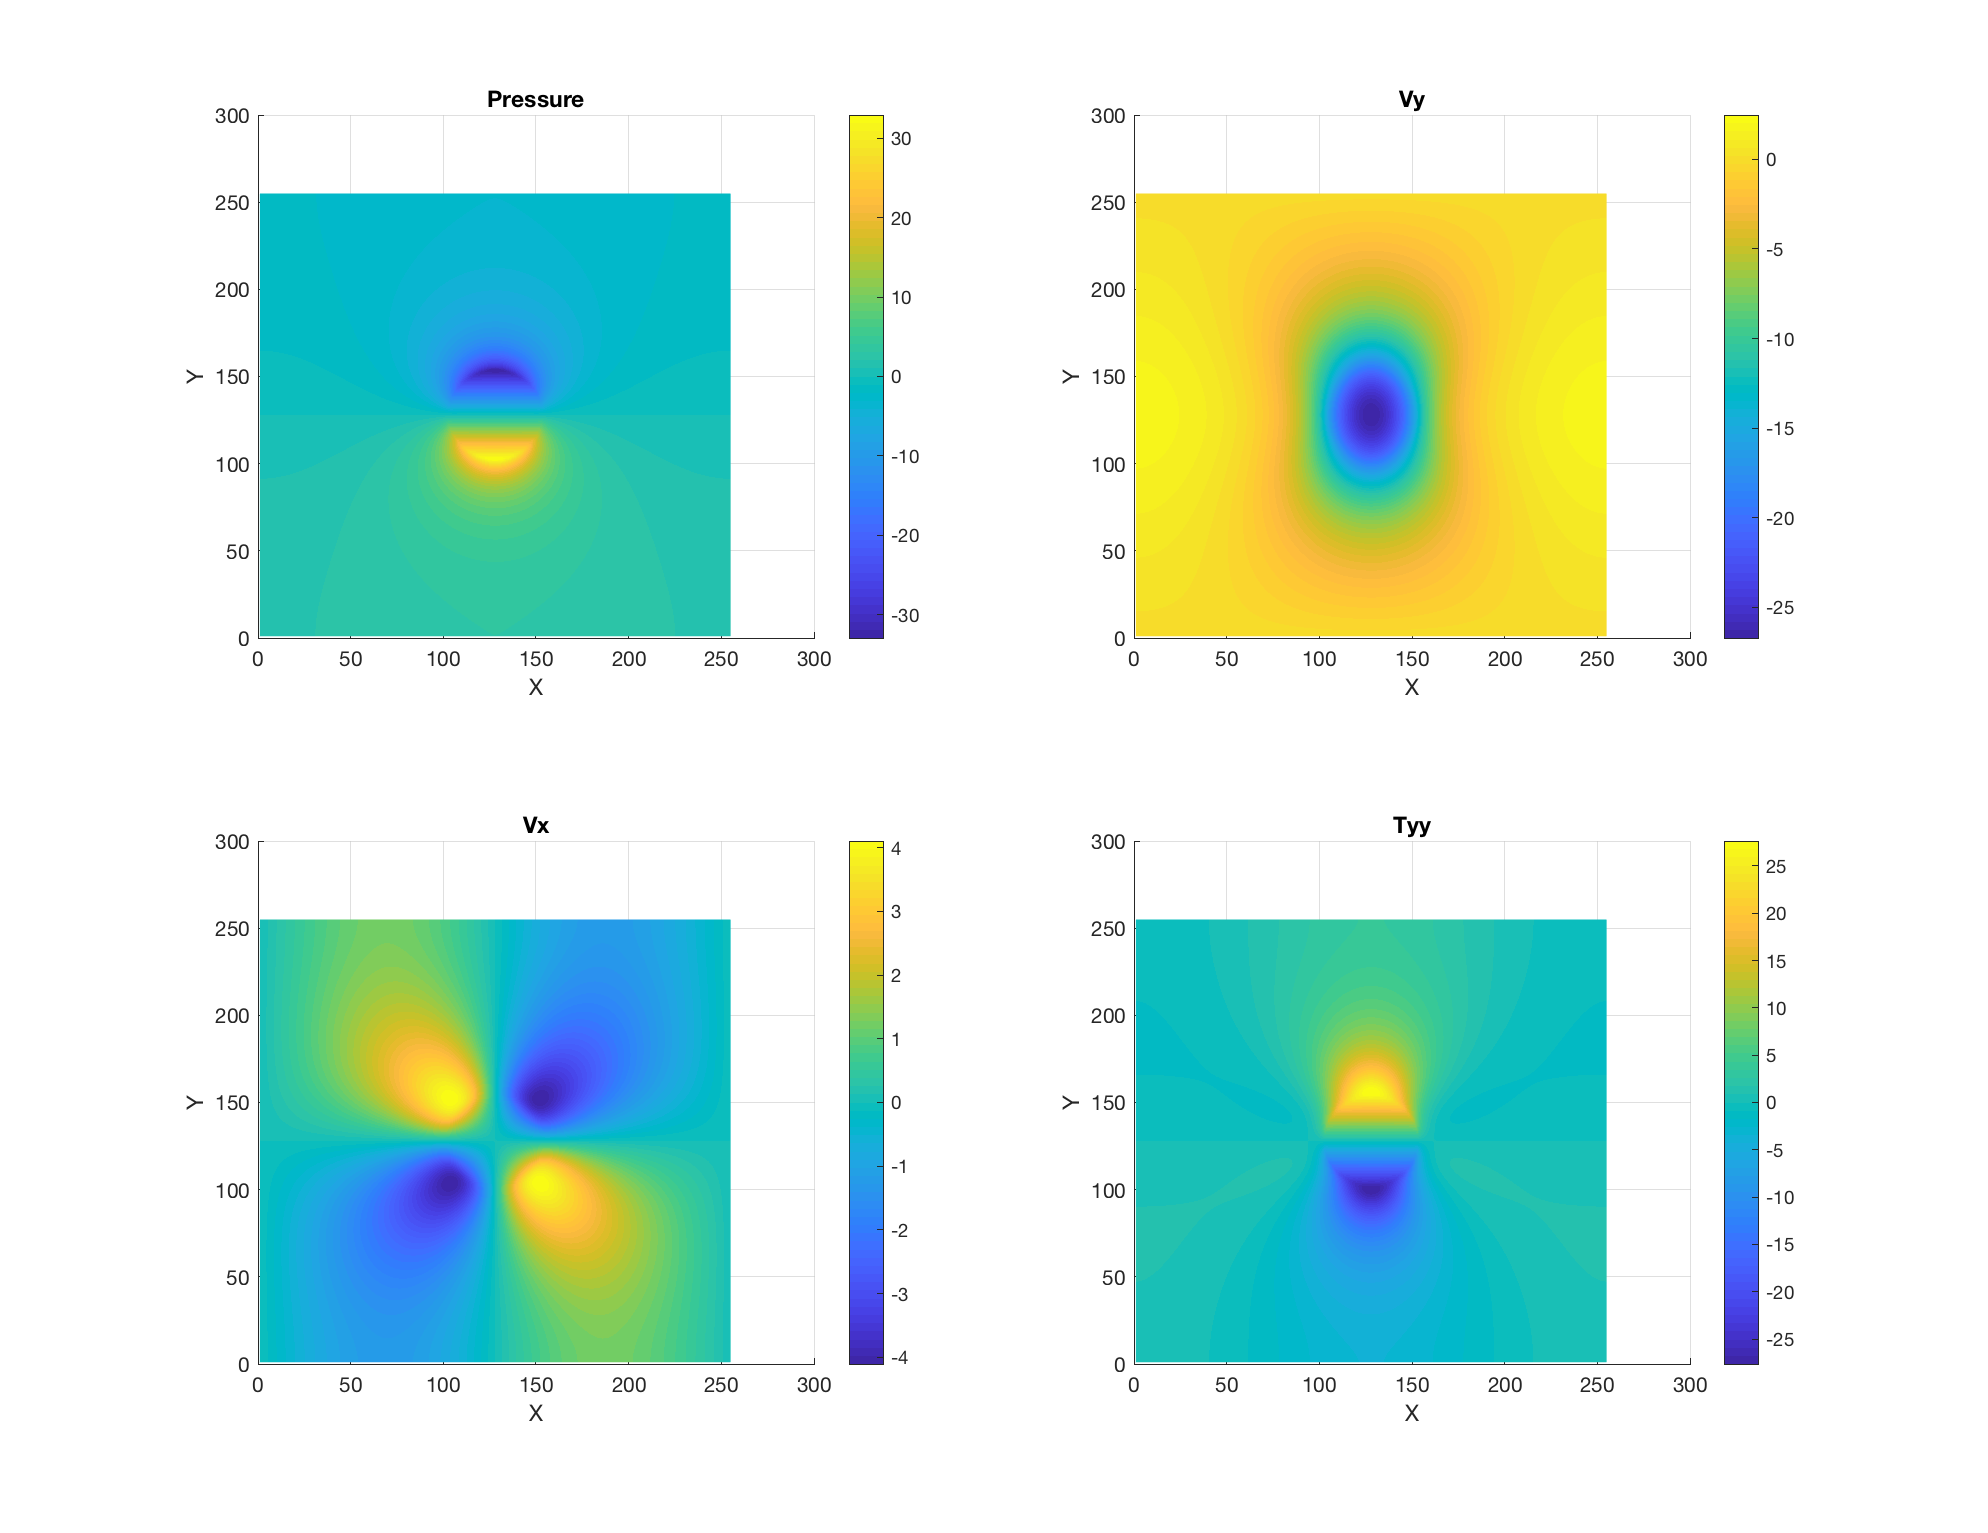
\includegraphics[width = .48\textwidth]{../3dvis/plots2d.png}
	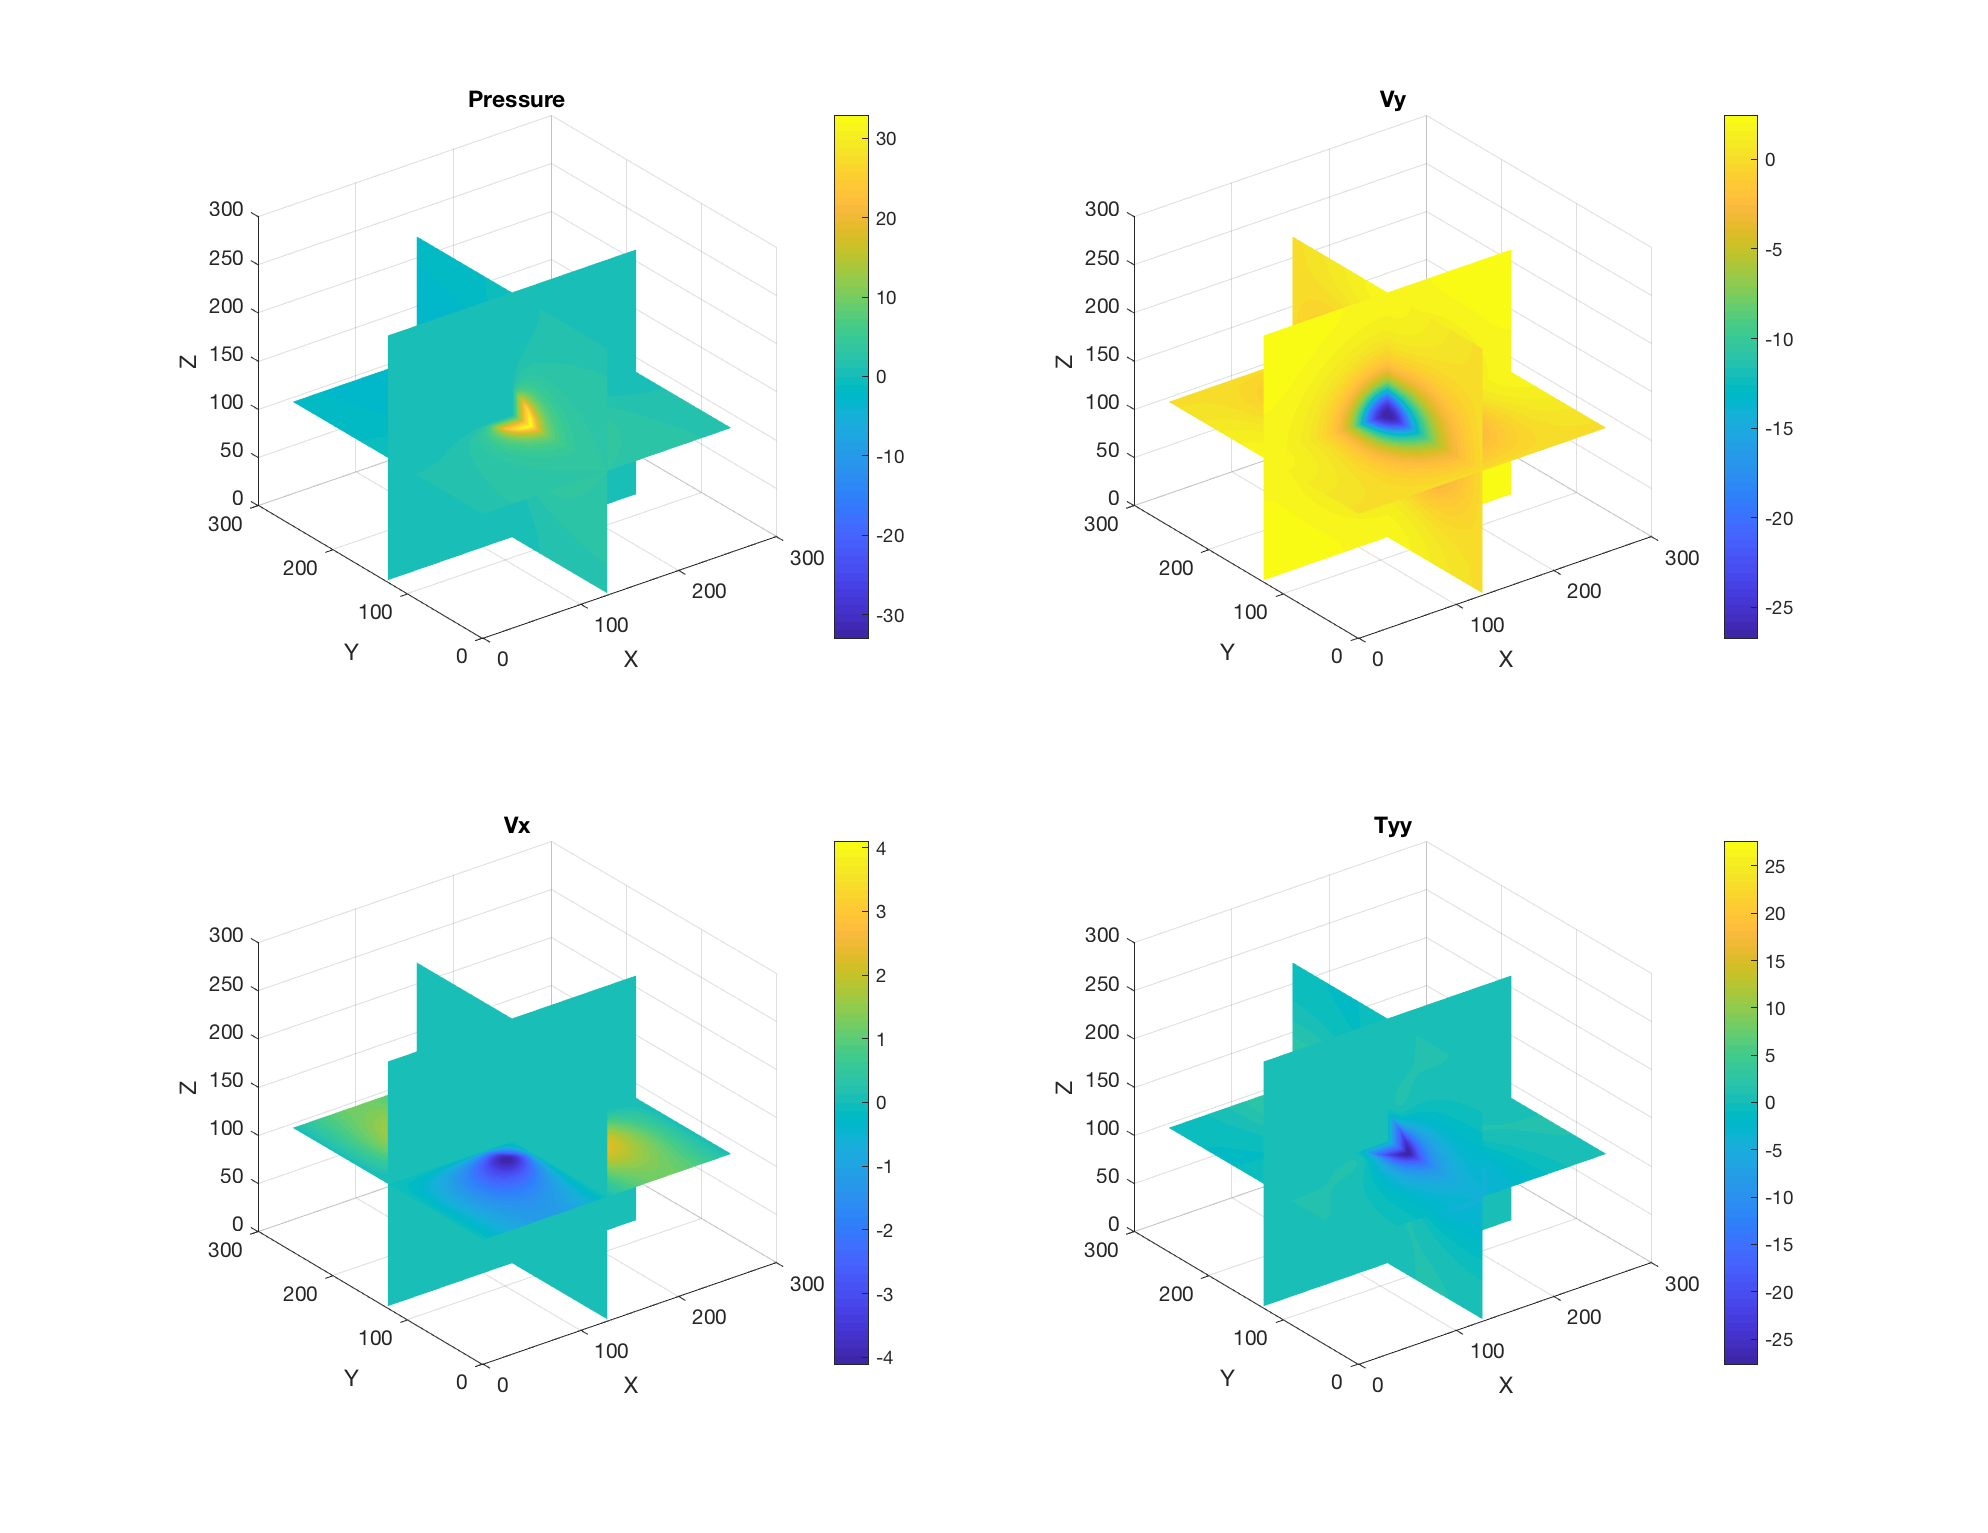
\includegraphics[width = .48\textwidth]{../3dvis/plots.png}
	\caption{\myfont 2D Cross section and 3D plot of final solution (255x255x255 run) of final solution (255x255x255 run)
}
\end{center}
\end{figure}


\begin{figure}[h!]
\begin{center}
	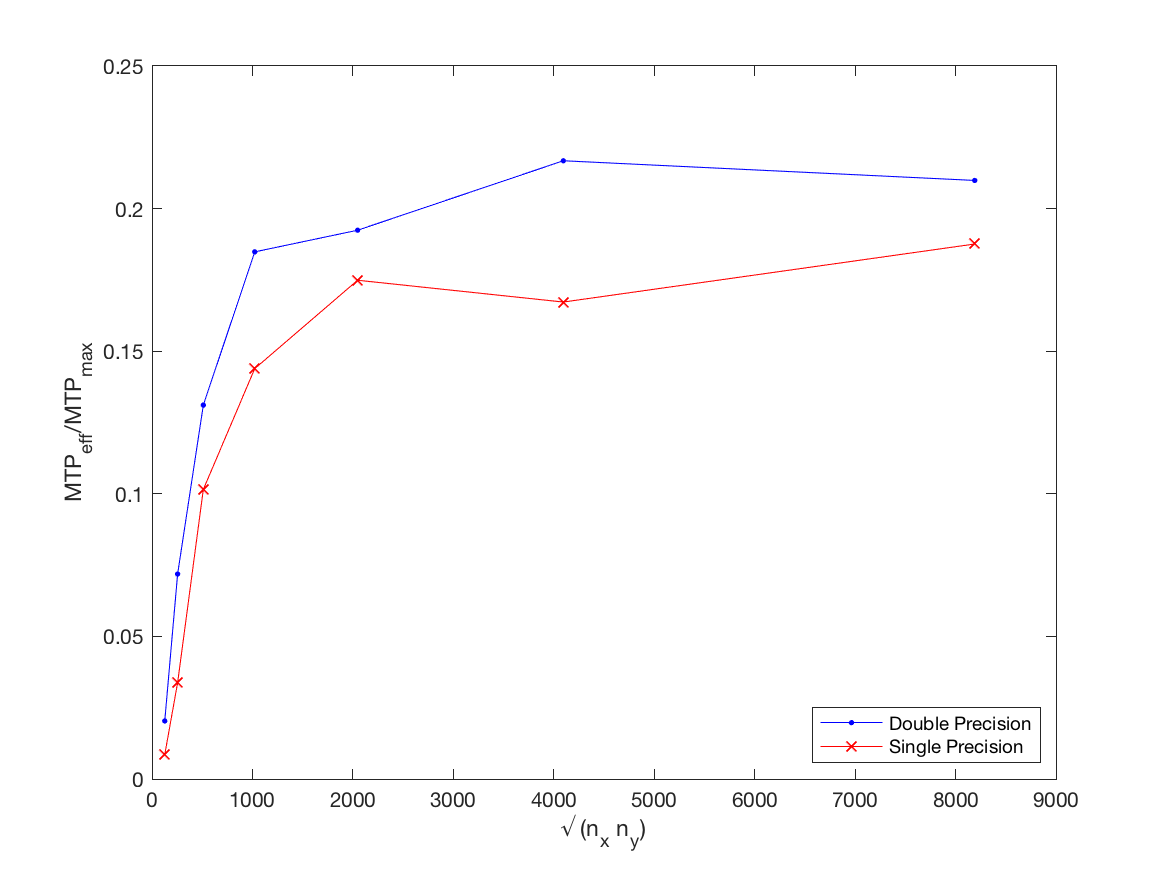
\includegraphics[width = .6\textwidth]{../3dvis/runTimes.png}
	\caption{\myfont MTP Plot. We see nice saturation up to a peak value close to MTP\textsubscript{max} after at a size of around 100 per axis. This value is slightly over the max theoretical, which suggests that this value is likely slightly mis-calibrated, this is discussed more below.}
	\label{fig:mtp}
\end{center}
\end{figure}

\begin{figure}[h!]
\begin{center}
	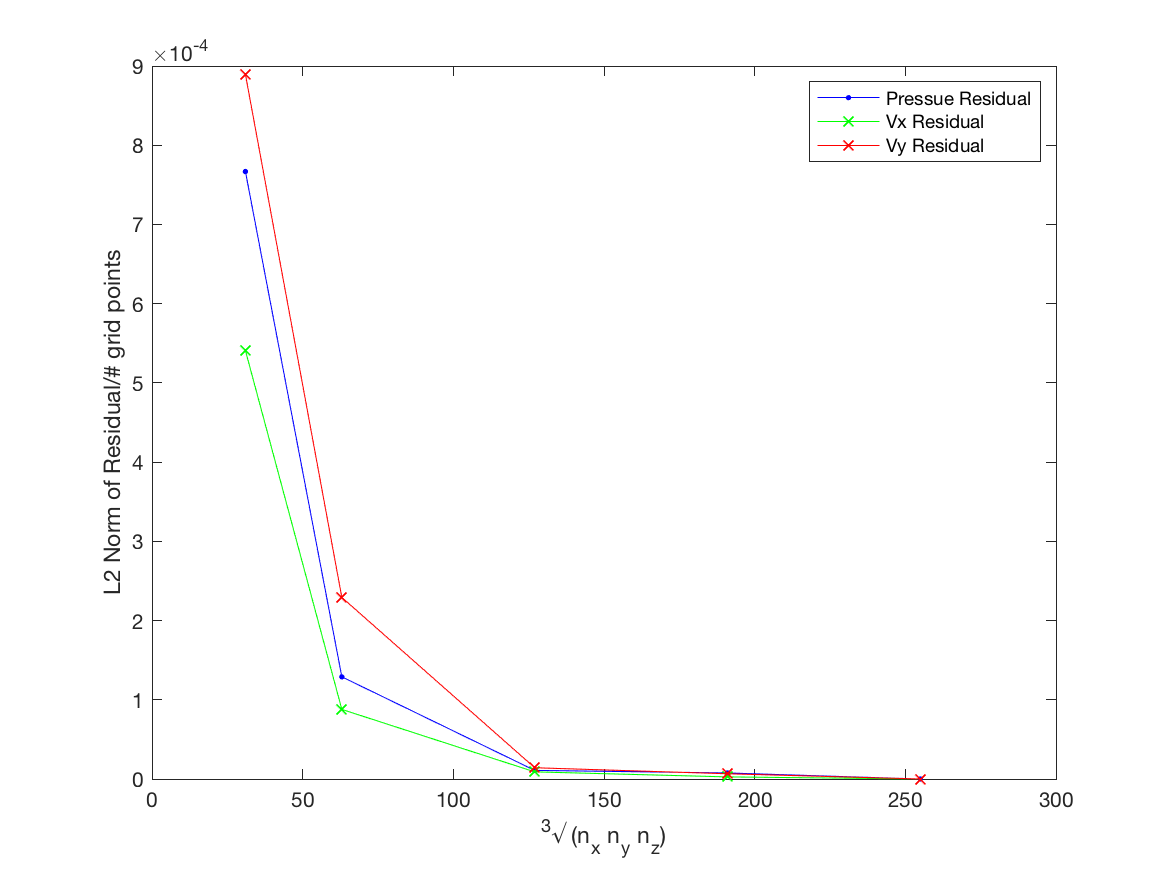
\includegraphics[width = .6\textwidth]{../3dvis/resids.png}
	\caption{\myfont Convergence with resolution increase. We see nice conversion to the peak resolution run. We take the 255x255x255 run to be ground truth for this convergence test.}
	\label{fig:conv}
\end{center}
\end{figure}

\begin{figure}[h!]
\begin{center}
	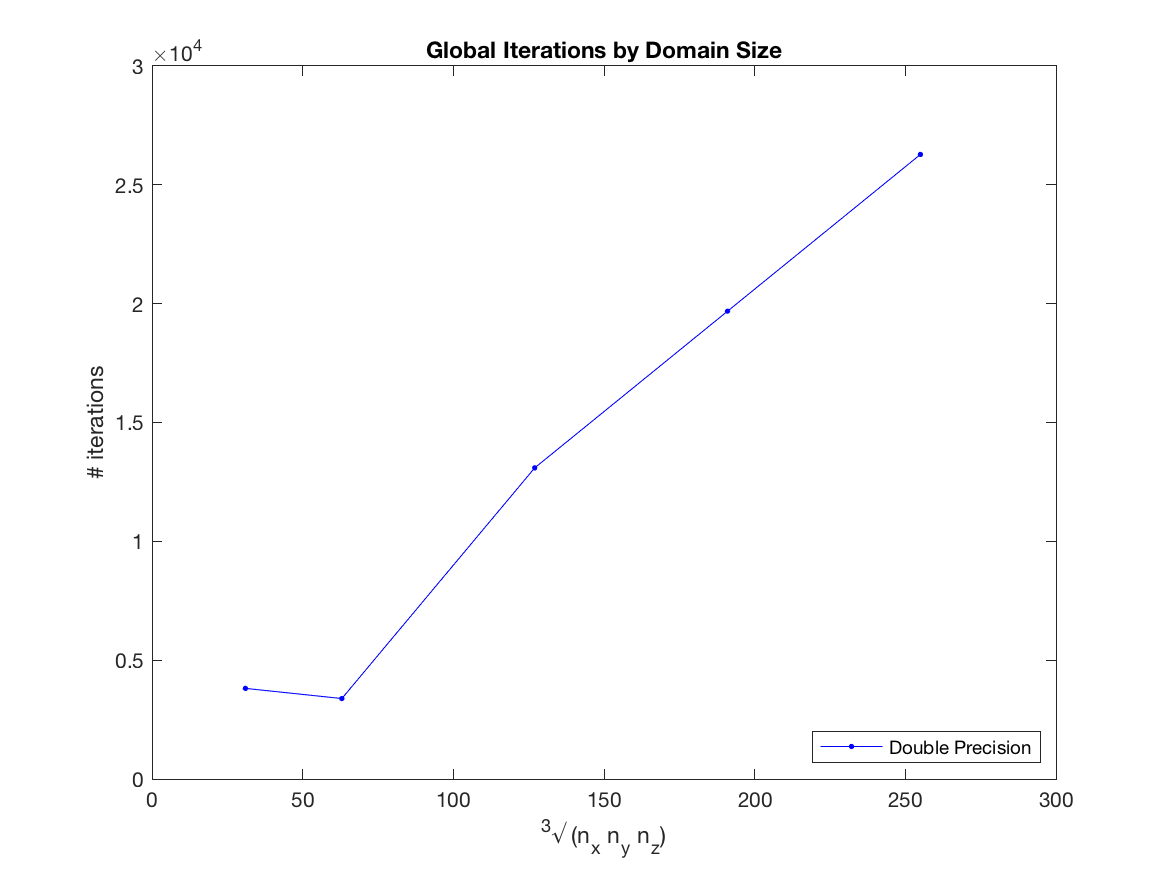
\includegraphics[width = .6\textwidth]{../3dvis/iterations.png}
	\caption{\myfont Convergence check in code, plot of iterations to converge. We see a nice linear trend in iterations needed to converge as grid size grows. This linear trend is confirmation that our accelerated pseudo-time convergence approach is working as desired.}
	\label{fig:its}
\end{center}
\end{figure}
% section results (end)
\section*{\myfont Discussion} % (fold)
We show that GPU parallelization can rapidly increase the run time of a simple forward finite difference code. We can see that the method is stable and converges to a unique solution as resolution increases as seen in the figure \ref{fig:conv}, and that the number of iterations to reach stabilization linearly increases with grid size in figure \ref{fig:its}. We also see that our code is likely memory bounded, as it saturates to (slightly over) MTP\textsubscript{max}. This over 100\% utilization likely comes from a mis-calibration in my code. I am calculating the MTP as if all 20 of the grid wide variables are re-written every iteration, when I suspect this is likely not the case, and that actual MTP saturates at roughly 80-90\% of MTP\textsubscript{max}. 
In contrast to more sophisticated matrix methods, this simple framework is easily expanded to include additional coupling factors like non-linear viscosity, thermomechanical coupling and anisotropy to name a few. Personally, this method could be very useful for modeling non-linear ice rheology and thermomechanic coupling over complex topography, though better boundary conditions would be needed for the topographic effects. I'm interested in extending this CUDA model to possibly include these additional physics as a part of my future research.
% section discussion (end)
\section*{\myfont Conclusion} % (fold)
In conclusion, we've demonstrated that a iterative GPU code can quickly and consistently solve a 3D viscous fluid flow scenario. Additionally, We point out how this simple iterative method could easily be adapted to introduce additional physics. We present the outputs of our 3D code, as well as plots showing convergence to the highest resolution case. Additionally, we show the linear growth in number of iterations to stabilize with number of grid points, which makes our method a potential option for larger scale simulations.
% section conculsion (end)
\end{document}
